\chapter{Конструкторская часть}

В данном разделе разработаны схемы реализаций алгоритма поиска всех вхождений подстроки в файле.

\section{Требования к ПО}

К программе предъявлен ряд требований:

\begin{itemize}[label=---]
	\item должен присутствовать интерфейс для выбора действий;
	\item должна работать с нативными потоками;
	\item должна замерять реальное время, затрачиваемое на работу реализаций алгоритмов.
\end{itemize}

\section{Требования к замерам времени}

Процессорное время — это время, которое процессор тратит на выполнение задачи или программы.
Оно измеряется в тактах процессора.

В данной лабораторной работе необходимо найти реальное время работы программы.
Так как в данной работе используется многопоточность, будет возникать необходимость блокировать работу потоков на мьютексах или семафорах.
Это время также необходимо учитывать при сравнении многопоточной и однопоточной реализации, несмотря на то, что поток не выполняет никаких действий в это время.

Для этого необходимо замерить реальное время, прошедшее от начала работы главного потока и до конца его выполнения.

\section{Разработка алгоритмов}

На рисунках \ref{fig:single} -- \ref{fig:writer} приведены схемы однопоточной и многопоточной версий алгоритма поиска подстроки в файле.

\begin{figure}[h]
	\centering
	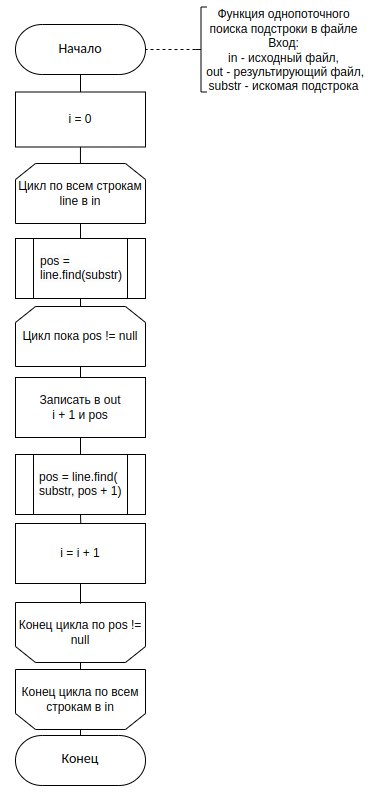
\includegraphics[width=0.65\textwidth]{img/single.png}
	\caption{Схема однопоточного алгоритма поиска подстроки в файле}
	\label{fig:single}
\end{figure}

\clearpage

\begin{figure}[h]
	\centering
	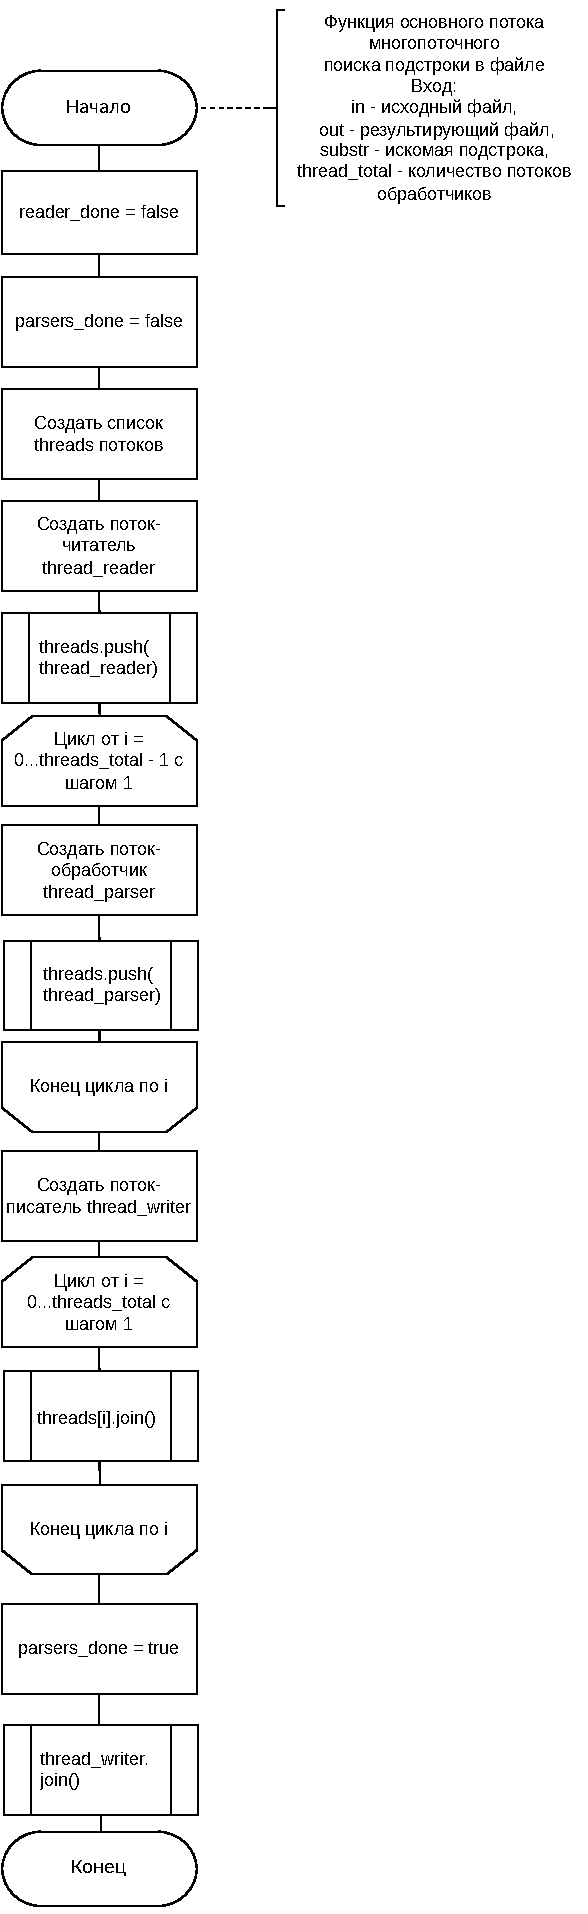
\includegraphics[height=0.9\textheight]{img/threads_main.pdf}
	\caption{Схема алгоритма работы основного потока, запускающего вспомогательные потоки}
	\label{fig:parallel}
\end{figure}

\clearpage

\begin{figure}[h]
	\centering
	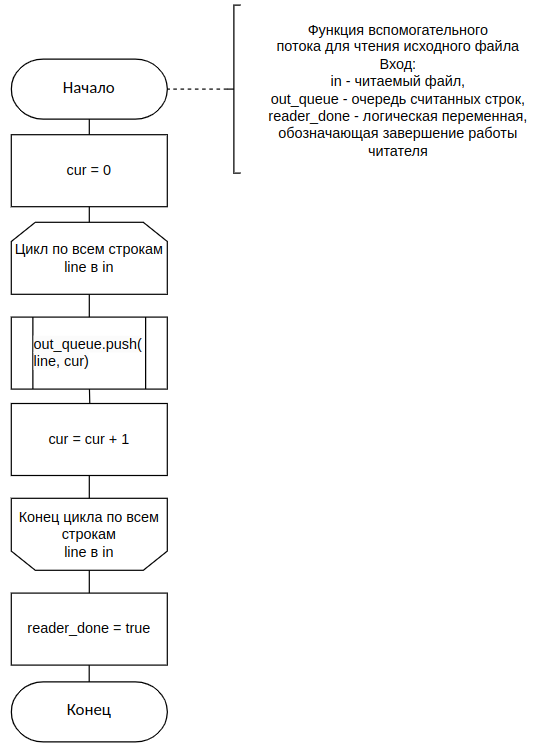
\includegraphics[height=0.8\textheight]{img/thread_reader.png}
	\caption{Схема алгоритма работы потока, выполняющего чтение из файла}
	\label{fig:thread_reader}
\end{figure}

\clearpage

\begin{figure}[h]
	\centering
	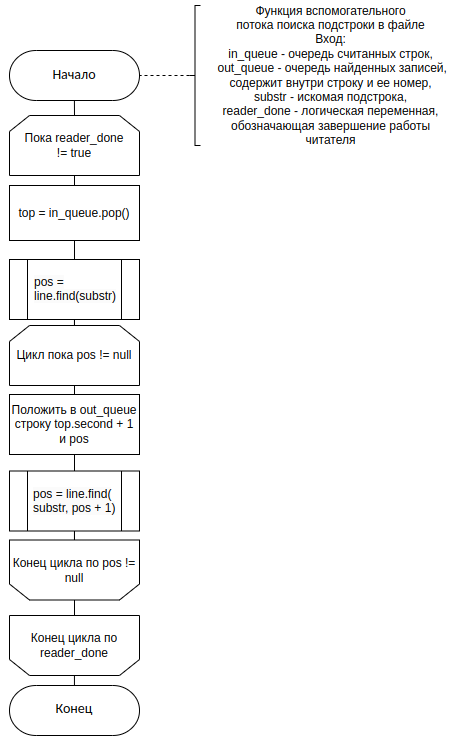
\includegraphics[height=0.8\textheight]{img/thread_substr.png}
	\caption{Схема алгоритма работы потока, обрабатывающего считанные строки}
	\label{fig:parser}
\end{figure}

\clearpage

\begin{figure}[h]
	\centering
	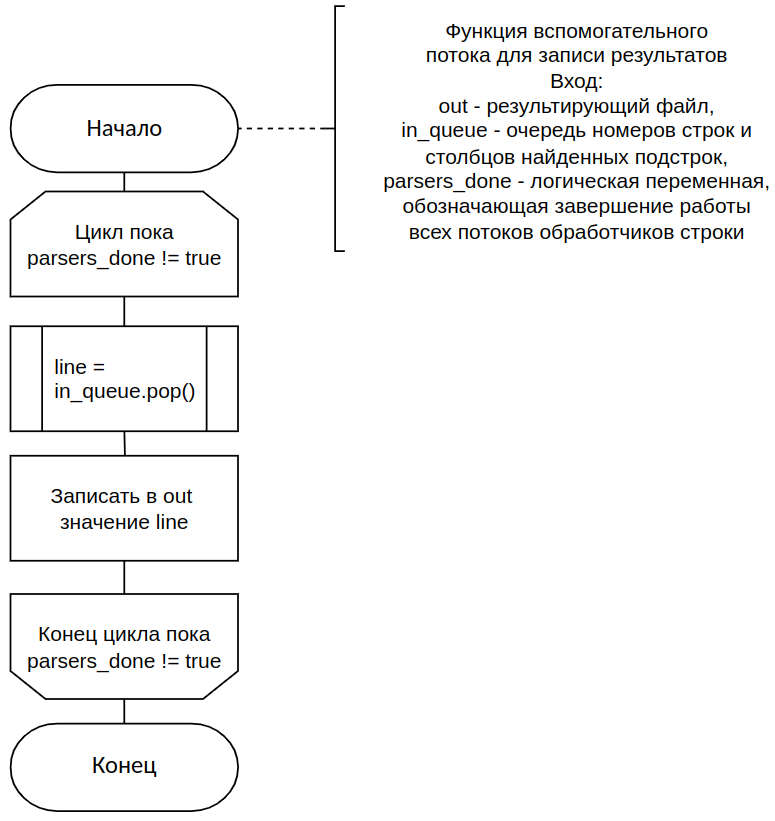
\includegraphics[height=0.6\textheight]{img/thread_writer.png}
	\caption{Схема алгоритма работы потока, записывающего результаты в файл}
	\label{fig:writer}
\end{figure}

\section*{Вывод}

В данном разделе разработаны схемы версий рассматриваемого алгоритма
